%% This is an example first section.  You should put section/appendix that you
%% write into a separate file, and add a line \include{yourfilename} to
%% main.tex, where `yourfilename.tex' is the name of the section/appendix file.
%% You can process specific files by typing their names in at the
%% \files=
%% prompt when you run the file main.tex through LaTeX.
\mysection{Introduction}

%\mysubsection{Problem Overview}

Digital devices are increasingly common in everyday life. Examples
include cell phones, modems, CD players, and high definition
televisions. These products utilize Digital Signal Processing (DSP)
for a variety of applications, including signal compression and
decompression, noise reduction, and error correction.  Because such
programs often run in embedded environments with limited power and
strict real-time requirements, this is a domain where optimization is
still very important.

Unfortunately, DSP optimizations typically defy high level language
compiler analysis.  Consequently, DSP applications must be hand-coded
or at the very least fine-tuned at the assembly level. This leads to a
host of problems: DSP experts must spend valuable hours writing
optimized low level code; every change in the design of the
application necessitates rewriting the code; the optimizations are
typically architecture-dependent, hence they are not portable or
robust.  These factors indicate that there is a need to effectively
analyze DSP applications and to automate their optimization in a
compiler.

In this paper, we introduce a new framework for analyzing and
optimizing a large class of DSP applications.  The framework, which we
call linear state space analysis, applies a large body of work on
linear state space systems to the domain of programming languages and
compilers.  A state space system is one in which a computational
element produces and consumes some values on each execution.  In
addition, some internal data may be preserved between executions; we
refer to these values as {\it states}.

A state space system is linear if it satisfies two criteria.  First,
each output must be a linear combination of the inputs and the current
state values.  Second, on each execution, the state values must be
updated as a linear combination of the inputs and the previous state
values.  Linear state space systems can model a large class of DSP
operations, including FIR filters, IIR filters, DCTs, upsamplers /
downsamplers and linear difference equations.  They are a
generalization of linear systems, in which a linear input-output
relationship holds but there is no state retained between executions.
There is a strong theoretical foundation for reasoning about linear
state space systems; it has been shown, for example, how to minimize
the number of states~\cite{Moore} as well as the number of parameters
in the system~\cite{Ackermann/Bucy,Mayne,Schutter}.

Our technique leverages domain-specific knowledge of linear state
space systems to perform novel optimization of stream programs.  Our
framework applies to languages based on the synchronous dataflow model
of computation.  In this model, a program is a set of autonomous
filters that communicate over FIFO channels.  On each execution, a
filter consumes some items from its input channels and produces some
items on its output channels; it may also retain states between
executions.  A filter can be modeled as a linear state space system if
it satisfies the criteria above.  In this paper, we use StreamIt as
the input language; StreamIt is a high-level language and compiler
infrastructure for DSP applications.

This paper makes the following contributions:

\begin{itemize}

\vspace{\itemshrink} \item An extraction algorithm that examines each
filter and, where possible, builds a state space representation to
describe its behavior.

\vspace{\itemshrink} \item Rules for combining adjacent state space
blocks into a single representation, thereby eliminating redundant
computations and enabling further optimizations.  Each possible
configuration of blocks (sequential, parallel, and cyclic) is handled.

\vspace{\itemshrink} \item A state removal optimization that detects
and eliminates redundant states within a block.

\vspace{\itemshrink} \item A parameter reduction optimization that
adjusts the coefficients of the state update and output calculation in
order to decrease the number of operations used.

\vspace{\itemshrink} \item An implementation of the above techniques
in the StreamIt compiler, with an evaluation over a small set of
benchmarks.  We demonstrate that state space analysis is more general
and can offer speedups over linear optimizations alone.

\vspace{\itemshrink} \end{itemize}

In the rest of this section, we give an overview of StreamIt and
illustrating examples of state space analysis\footnote{As the rest of
this paper is devoted to linear state space analysis, we often say
only ``state space analysis'' for brevity.}.
Section~\ref{sec:statespace} gives the details of our state space
representation, including extraction and combination rules, while
Section~\ref{sec:optimization} describes the optimizations.  In
Section~\ref{sec:results} we discuss our implementation and results.
Section~\ref{sec:related} details related work, and
Section~\ref{sec:conclusion} concludes.

%% A linear state space system is one in which a computational element
%% produces and consumes some values on each execution.  In addition,
%% some internal data may be preserved between executions; we refer to
%% these values as {\it states}.  In a linear state space system, each
%% output is a linear combination of the states and the input values.
%% The states are also updated on each execution to be a linear
%% combination of the inputs and the previous state values.  There is a

%% \mysubsection{DSP Analysis}

%%     In order to properly analyze DSP applications, we must use an
%% appropriate framework to model them.  This framework should
%% contain a number of simplifications in order to make our analysis
%% workable, but not too many simplifications that our analysis fails
%% to be robust.

%%     We start with the top level notion of an
%% application, defined as a large module that receives inputs,
%% performs computations, and outputs results.  This definition,
%% while correct, does not lend itself to any type of application
%% analysis. The first simplification we make is to divide an
%% application into blocks, which are abstract input-output modules.
%% These blocks are interconnected in a certain way to form the full
%% application. We can think of each block as a mini-application: it
%% takes its own inputs, performs calculations, and produces outputs.

%% \begin{figure}[t]
%%   \centering
%%   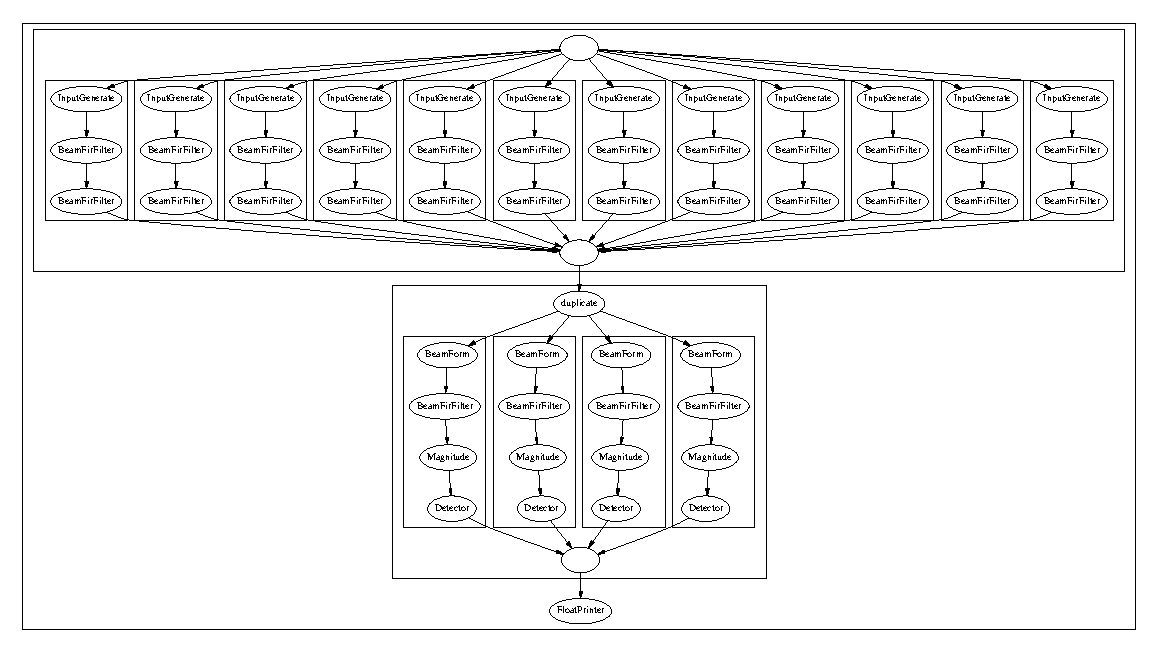
\includegraphics[width=5.0in]{figures/beamformer.eps}
%%   \caption{A DSP block diagram of the application Beamformer}
%%   \label{fig:block-diagram}
%% \end{figure}

%%     Blocks can be characterized in various ways. The simplest characterization
%% of blocks is a \textit{linear} block, defined as a module that
%% outputs a linear combination of its inputs plus a constant term. A
%% linear block can be represented by a matrix relating inputs to
%% outputs and a vector of constants. The next simplest
%% characterization of blocks is \textit{linear state space}. Such a
%% block uses a set of state variables. The output of this block is a
%% linear combination of its inputs and state variables. In addition,
%% the state variables are updated by a linear combination of
%% themselves and inputs.  A linear state space block can be
%% represented by four independent matrices.

%%     A linear state space characterization is more general than a
%% linear characterization - all linear blocks are also linear
%% state space blocks, but the converse is not true. The intuitive
%% reason for this fact is that a linear block is memoryless, meaning
%% the outputs only depend on current inputs. However, a linear
%% state space block has memory in the form of state variables, so
%% the outputs depend on current inputs and past inputs.

%%     We will perform analysis and optimization of DSP applications at
%% the linear state space level. We choose this representation
%% because it models a wide class of applications or parts of
%% applications, and it is simple to work with.

%%     Our work with state space representations will be done in the
%% context of StreamIt, a programming language designed for streaming
%% applications \cite{streamitcc}.  StreamIt allows users to create
%% their own blocks, but limits the way these blocks can be
%% connected. We perform the following steps on a StreamIt program:

%% \begin{enumerate}
%% \vspace{\itemshrink} \item Examine each block and determine whether or not it can be
%% characterized as linear state space. If it can, extract the
%% appropriate state space representation.

%% \vspace{\itemshrink} \item Combine connected blocks that each have a state space
%% representation, using an appropriate set of rules depending on the
%% type of connection.

%% \vspace{\itemshrink} \item Optimize representations through the use of state space
%% transformations.

%% \vspace{\itemshrink} \item Convert the state space representation(s) back to StreamIt
%% code.
%% \vspace{\itemshrink} \end{enumerate}

%% \mysubsection{Organization}
